% fig_performance_comparison.tex - Bar chart comparing propulsion technologies
% Standalone compilation: pdflatex fig_performance_comparison.tex
\documentclass[tikz,border=5pt]{standalone}
\usepackage{pgfplots}
\usepackage{amsmath}
\pgfplotsset{compat=1.18}
\usepgfplotslibrary{groupplots}

\begin{document}
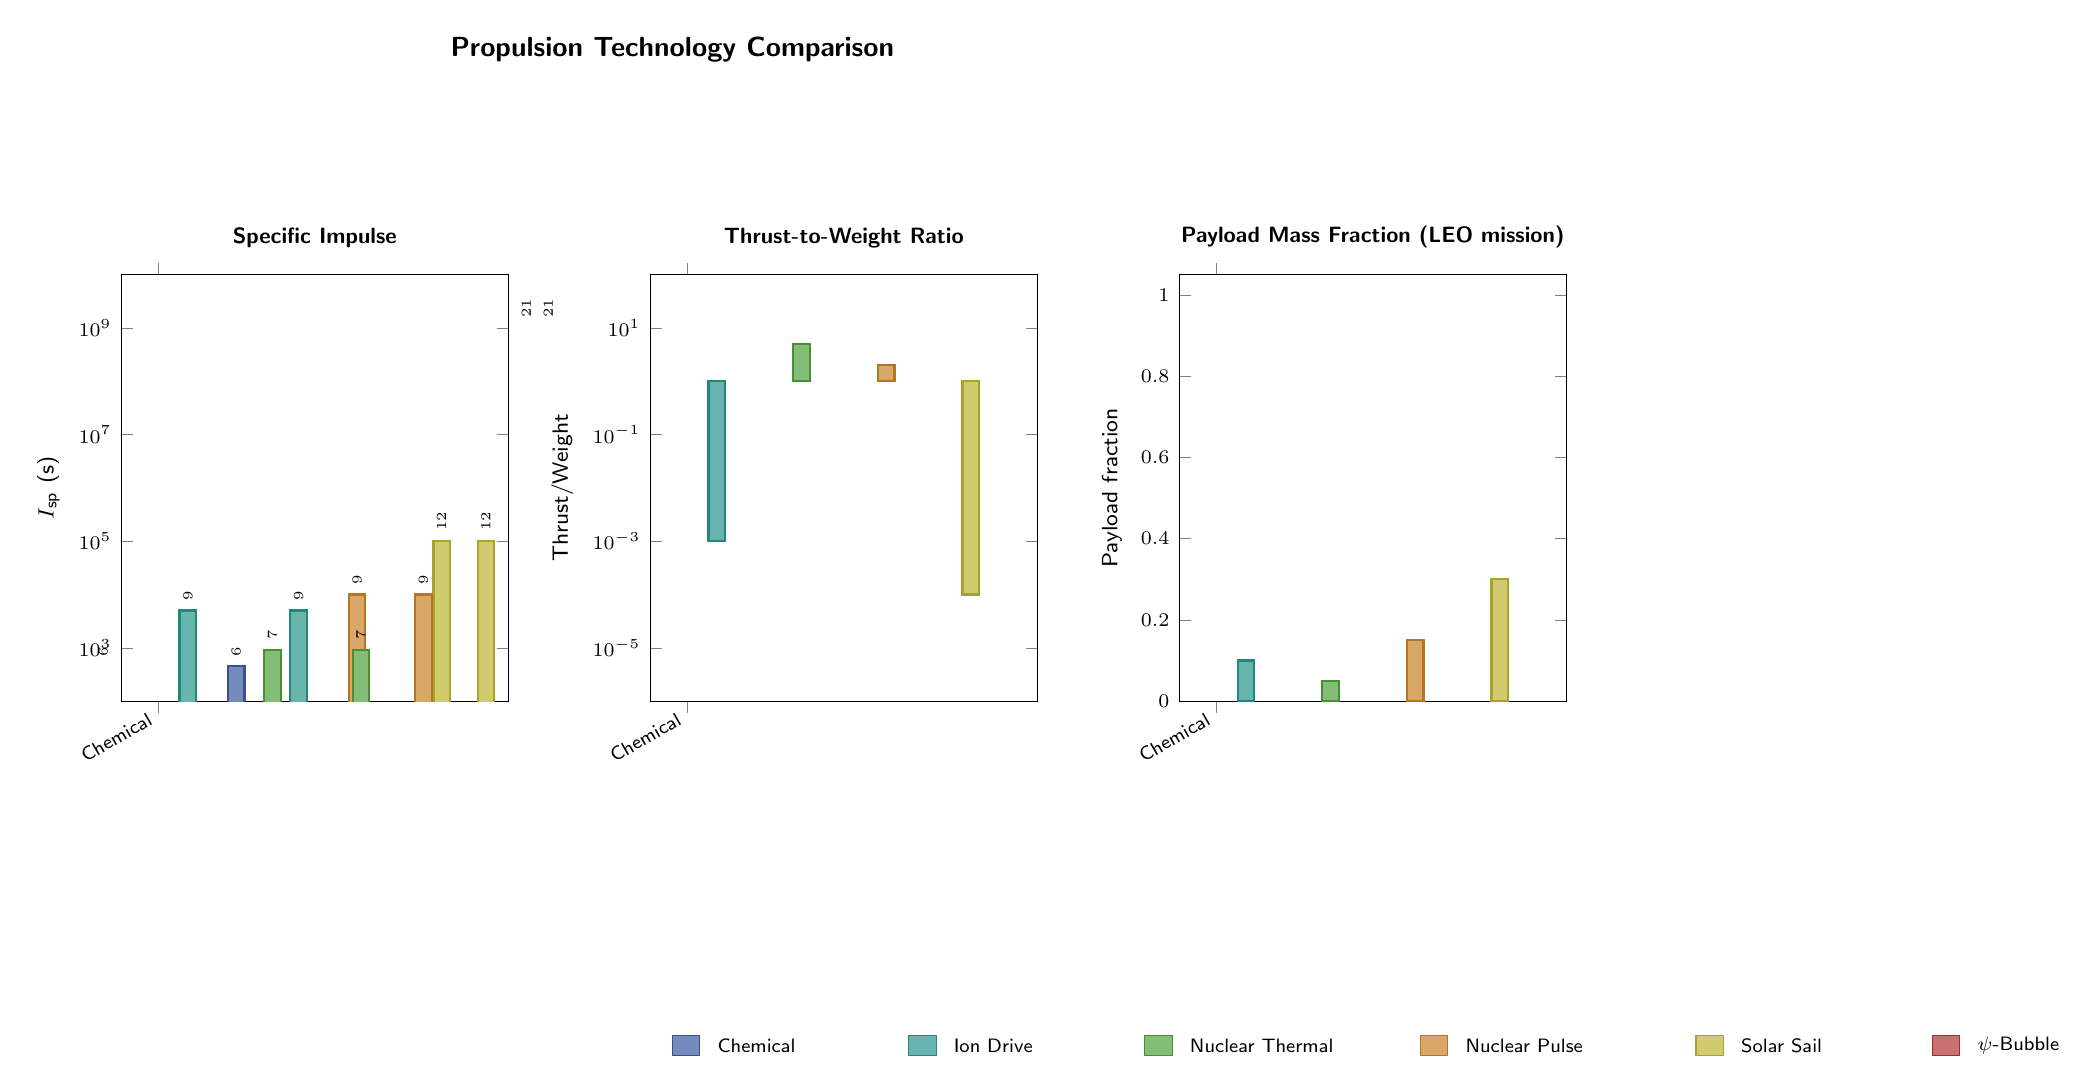
\begin{tikzpicture}

\definecolor{chemBlue}{RGB}{60,90,160}
\definecolor{ionTeal}{RGB}{40,150,140}
\definecolor{ntGreen}{RGB}{80,160,60}
\definecolor{npOrange}{RGB}{200,130,40}
\definecolor{sailYellow}{RGB}{190,180,50}
\definecolor{psiRed}{RGB}{180,50,50}

\pgfplotsset{
    techbar/.style={
        ybar,
        bar width=6pt,
        enlarge x limits=0.12,
        ylabel style={font=\footnotesize\sffamily},
        xlabel style={font=\footnotesize\sffamily},
        tick label style={font=\scriptsize\sffamily},
        title style={font=\footnotesize\sffamily\bfseries},
        legend style={
            font=\scriptsize\sffamily,
            at={(0.5,-0.35)},
            anchor=north,
            legend columns=3,
            column sep=4pt,
            /tikz/every even column/.append style={column sep=8pt},
        },
        symbolic x coords={Chemical, Ion, Nuc.~Thermal, Nuc.~Pulse, Solar Sail, $\psi$-Bubble},
        xtick=data,
        x tick label style={rotate=30, anchor=east, font=\scriptsize\sffamily},
        nodes near coords style={font=\tiny\sffamily, rotate=90, anchor=west},
        every axis plot/.append style={thick},
    }
}

\begin{groupplot}[
    group style={
        group size=3 by 1,
        xlabels at=edge bottom,
        horizontal sep=1.8cm,
    },
    techbar,
    width=6.5cm, height=7cm,
]

% --- Panel 1: Specific Impulse (log scale) ---
\nextgroupplot[
    ymode=log,
    ymin=100, ymax=1e10,
    ylabel={$I_\text{sp}$ (s)},
    title={Specific Impulse},
    nodes near coords={\pgfmathprintnumber[fixed,precision=0]{\pgfplotspointmeta}},
]
\addplot[fill=chemBlue!70, draw=chemBlue!90!black]
    coordinates {(Chemical,450) (Ion,0) (Nuc.~Thermal,0) (Nuc.~Pulse,0) (Solar Sail,0) ($\psi$-Bubble,0)};
\addplot[fill=ionTeal!70, draw=ionTeal!90!black]
    coordinates {(Chemical,0) (Ion,5000) (Nuc.~Thermal,0) (Nuc.~Pulse,0) (Solar Sail,0) ($\psi$-Bubble,0)};
\addplot[fill=ntGreen!70, draw=ntGreen!90!black]
    coordinates {(Chemical,0) (Ion,0) (Nuc.~Thermal,900) (Nuc.~Pulse,0) (Solar Sail,0) ($\psi$-Bubble,0)};
\addplot[fill=npOrange!70, draw=npOrange!90!black]
    coordinates {(Chemical,0) (Ion,0) (Nuc.~Thermal,0) (Nuc.~Pulse,10000) (Solar Sail,0) ($\psi$-Bubble,0)};
\addplot[fill=sailYellow!70, draw=sailYellow!90!black]
    coordinates {(Chemical,0) (Ion,0) (Nuc.~Thermal,0) (Nuc.~Pulse,0) (Solar Sail,100000) ($\psi$-Bubble,0)};
\addplot[fill=psiRed!70, draw=psiRed!90!black]
    coordinates {(Chemical,0) (Ion,0) (Nuc.~Thermal,0) (Nuc.~Pulse,0) (Solar Sail,0) ($\psi$-Bubble,1e9)};

% Combined single-tech bars
\addplot[fill=chemBlue!70, draw=chemBlue!90!black, forget plot]
    coordinates {(Chemical,450)};
\addplot[fill=ionTeal!70, draw=ionTeal!90!black, forget plot]
    coordinates {(Ion,5000)};
\addplot[fill=ntGreen!70, draw=ntGreen!90!black, forget plot]
    coordinates {(Nuc.~Thermal,900)};
\addplot[fill=npOrange!70, draw=npOrange!90!black, forget plot]
    coordinates {(Nuc.~Pulse,10000)};
\addplot[fill=sailYellow!70, draw=sailYellow!90!black, forget plot]
    coordinates {(Solar Sail,100000)};
\addplot[fill=psiRed!70, draw=psiRed!90!black, forget plot]
    coordinates {($\psi$-Bubble,1e9)};

% --- Panel 2: Thrust-to-Weight Ratio (log scale) ---
\nextgroupplot[
    ymode=log,
    ymin=1e-6, ymax=100,
    ylabel={Thrust/Weight},
    title={Thrust-to-Weight Ratio},
]
% Single bar per technology
\addplot[fill=chemBlue!70, draw=chemBlue!90!black]
    coordinates {(Chemical,30)};
\addplot[fill=ionTeal!70, draw=ionTeal!90!black]
    coordinates {(Ion,0.001)};
\addplot[fill=ntGreen!70, draw=ntGreen!90!black]
    coordinates {(Nuc.~Thermal,5)};
\addplot[fill=npOrange!70, draw=npOrange!90!black]
    coordinates {(Nuc.~Pulse,2)};
\addplot[fill=sailYellow!70, draw=sailYellow!90!black]
    coordinates {(Solar Sail,0.0001)};
\addplot[fill=psiRed!70, draw=psiRed!90!black]
    coordinates {($\psi$-Bubble,10)};

% --- Panel 3: Payload Mass Fraction ---
\nextgroupplot[
    ymin=0, ymax=1.05,
    ylabel={Payload fraction},
    title={Payload Mass Fraction (LEO mission)},
]
\addplot[fill=chemBlue!70, draw=chemBlue!90!black]
    coordinates {(Chemical,0.02)};
\addplot[fill=ionTeal!70, draw=ionTeal!90!black]
    coordinates {(Ion,0.10)};
\addplot[fill=ntGreen!70, draw=ntGreen!90!black]
    coordinates {(Nuc.~Thermal,0.05)};
\addplot[fill=npOrange!70, draw=npOrange!90!black]
    coordinates {(Nuc.~Pulse,0.15)};
\addplot[fill=sailYellow!70, draw=sailYellow!90!black]
    coordinates {(Solar Sail,0.30)};
\addplot[fill=psiRed!70, draw=psiRed!90!black]
    coordinates {($\psi$-Bubble,0.90)};

\end{groupplot}

% ============================================================
% SHARED LEGEND (manual, below all panels)
% ============================================================
\begin{scope}[yshift=-4.5cm, xshift=7cm]
    \foreach \col/\lab/\xoff in {
        chemBlue/Chemical/0,
        ionTeal/Ion Drive/3,
        ntGreen/Nuclear Thermal/6,
        npOrange/Nuclear Pulse/9.5,
        sailYellow/Solar Sail/13,
        psiRed/$\psi$-Bubble/16%
    } {
        \fill[\col!70] (\xoff,0) rectangle ++(0.35,0.25);
        \draw[\col!90!black] (\xoff,0) rectangle ++(0.35,0.25);
        \node[right, font=\scriptsize\sffamily] at ({\xoff+0.45},0.12) {\lab};
    }
\end{scope}

% ============================================================
% TITLE
% ============================================================
\node[font=\normalsize\sffamily\bfseries, anchor=south] at (7,8)
    {Propulsion Technology Comparison};

\end{tikzpicture}
\end{document}
